\chapter{Human-robot interaction}



\section{Introduction}

As robotic arms evolved from specialized operators capable of only executing a single task to complex structures with high computing power, humans became able to interact more closely with the machines.

Human-robot interaction (HRI) studies the means of communication between humans and robots by designing, understanding, and evaluating robotic systems that coexist with humans. It is a multidisciplinary field with contributions from human-computer interaction, artificial intelligence, robotics, natural-language understanding, design, and psychology.

Interaction can be separated into two general categories: remote and proximate. In remote interaction, the human and the robot are separated spatially, or even possibly temporally. Remote interaction can be \lstinline{teleoperation} if the robot is controlled by its interaction with the human as a general supervisor, or \lstinline{telemanipulation} if the human controls the robot completely via a physical manipulator.

In proximate interaction, communication is often more social, focusing on more abstract concepts such as emotions. The robot can perceive the human with sensibility to touch, for physical interaction; sight, for analyzing posture and facial signals; or hearing and speaking to communicate verbally like a real human.

We designed two interfaces for remote and proximate interaction. First, hand movement and gesture control, which allows the human to manipulate the robotic arm remotely by using their hand as a guide for the robot and making hand gestures to trigger actions. And second, voice control, a proximate interaction using natural language understanding to enable the robot to accept commands formulated in a natural, "human-like" manner.



\section{Related work}

Many technologies can be used to develop interactions due to the flexible nature of robotic platforms. From computer vision, to wearable electronics, to virtual reality, many things can be adapted to enable control of a robotic arm.

Using a Virtual Reality headset, Lipton et al. \cite{robot_control_vr} were able to create a platform for teleoperation, implementing tasks such as pick and place, assembly, and manufacturing. It takes inspiration from Penfield's Homunculus model \cite{penfield1950cerebral}, creating a mapping from human to robot enhancing sight and hand feeling.

Complete structures can also be constructed to place the user in a sort of "command chair", where they can precisely move the robot \cite{centauro} \ref{fig:centauro}.

\begin{marginfigure}
    \centering
    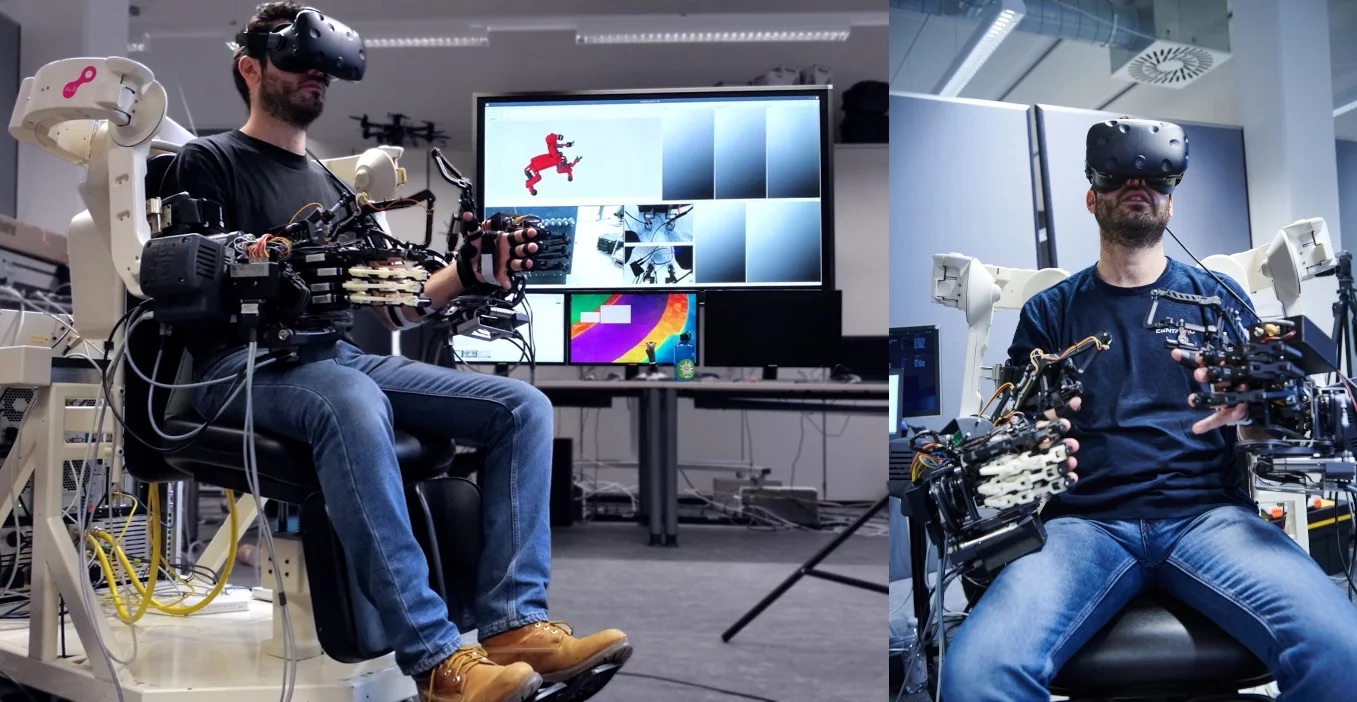
\includegraphics{images/centauro.png}
    \caption{Centauro project control chair}
    \label{fig:centauro}
\end{marginfigure}

To create a direct link between the robot brain and the human brain, Salazar-Gomez et al. \cite{robot_control_eeg} use an EEG (Electroencephalogram) headset to detect brain signals related to unexpected error making (ErrPs) to correct mistakes in classification tasks. It can change the behavior of a robotic arm when it is making a mistake during a task consisting of sorting object into different labelled bins.

The body itself can act as a control interface using wearable devices \cite{robot_gesture_control_wearable}. By measuring biceps, triceps and forearm activity, but also arm motion, DelPreto et al. were able to control a drone through obstacles using only their arm.

Interfaces can be used to explore the relationships between human and robot. By studying the emotional response of humans giving an object to a robot, and the robot taking the object in different manners, we can, for example, find the characteristics of robotic movements that make them more trustworthy in the eyes of humans, to make them more socially apt, and to mimic human-human interactions \cite{robot_handoff}.

There are also ways of controlling a robot that don't involve physical contact or devices. Matarneh et al. \cite{matarneh_maksymova_deineko_lyashenko_1970} used a deep learning algorithm, specifically a multi-layer perceptron, to interpret voice into commands. With these commands, researchers were able to control the movements of the robot directly from voice data, while other solutions involve translating voice into text first, and then text into commands \cite{Janicek_2021}.



\section{Hand movement and gesture control}


\subsection{Introduction}

A robotic arm closely mimics the workings of the human arm, with joints and muscles in the form of motors. It is not surprising, then, that we would want to create a link between the human arm and the robot arm. On another level, grasping tasks are some of the most common tasks of a robotic arm, just like the hand of the human.

These are the reasons why we created hand movement and gesture control for ALFRED. By mirroring the robot and human arms, we can create a strong connection between machine and operator. We can take advantage of the dexterity of the hand and translate this dexterity into the robotic arm by interpreting complex hand gestures into commands for the robot. Hand movement and gesture control can be used as a remote interface, making the robotic arm act as the user's arm in another place, or as a proximate interface, acting like a mirror showing a robotic image of the user to aid them in their current task.


% \subsection{Related work}

% % XXX: related_work


\subsection{Contribution}

\subsubsection{Concept}

\begin{figure}[h]
    \centering
    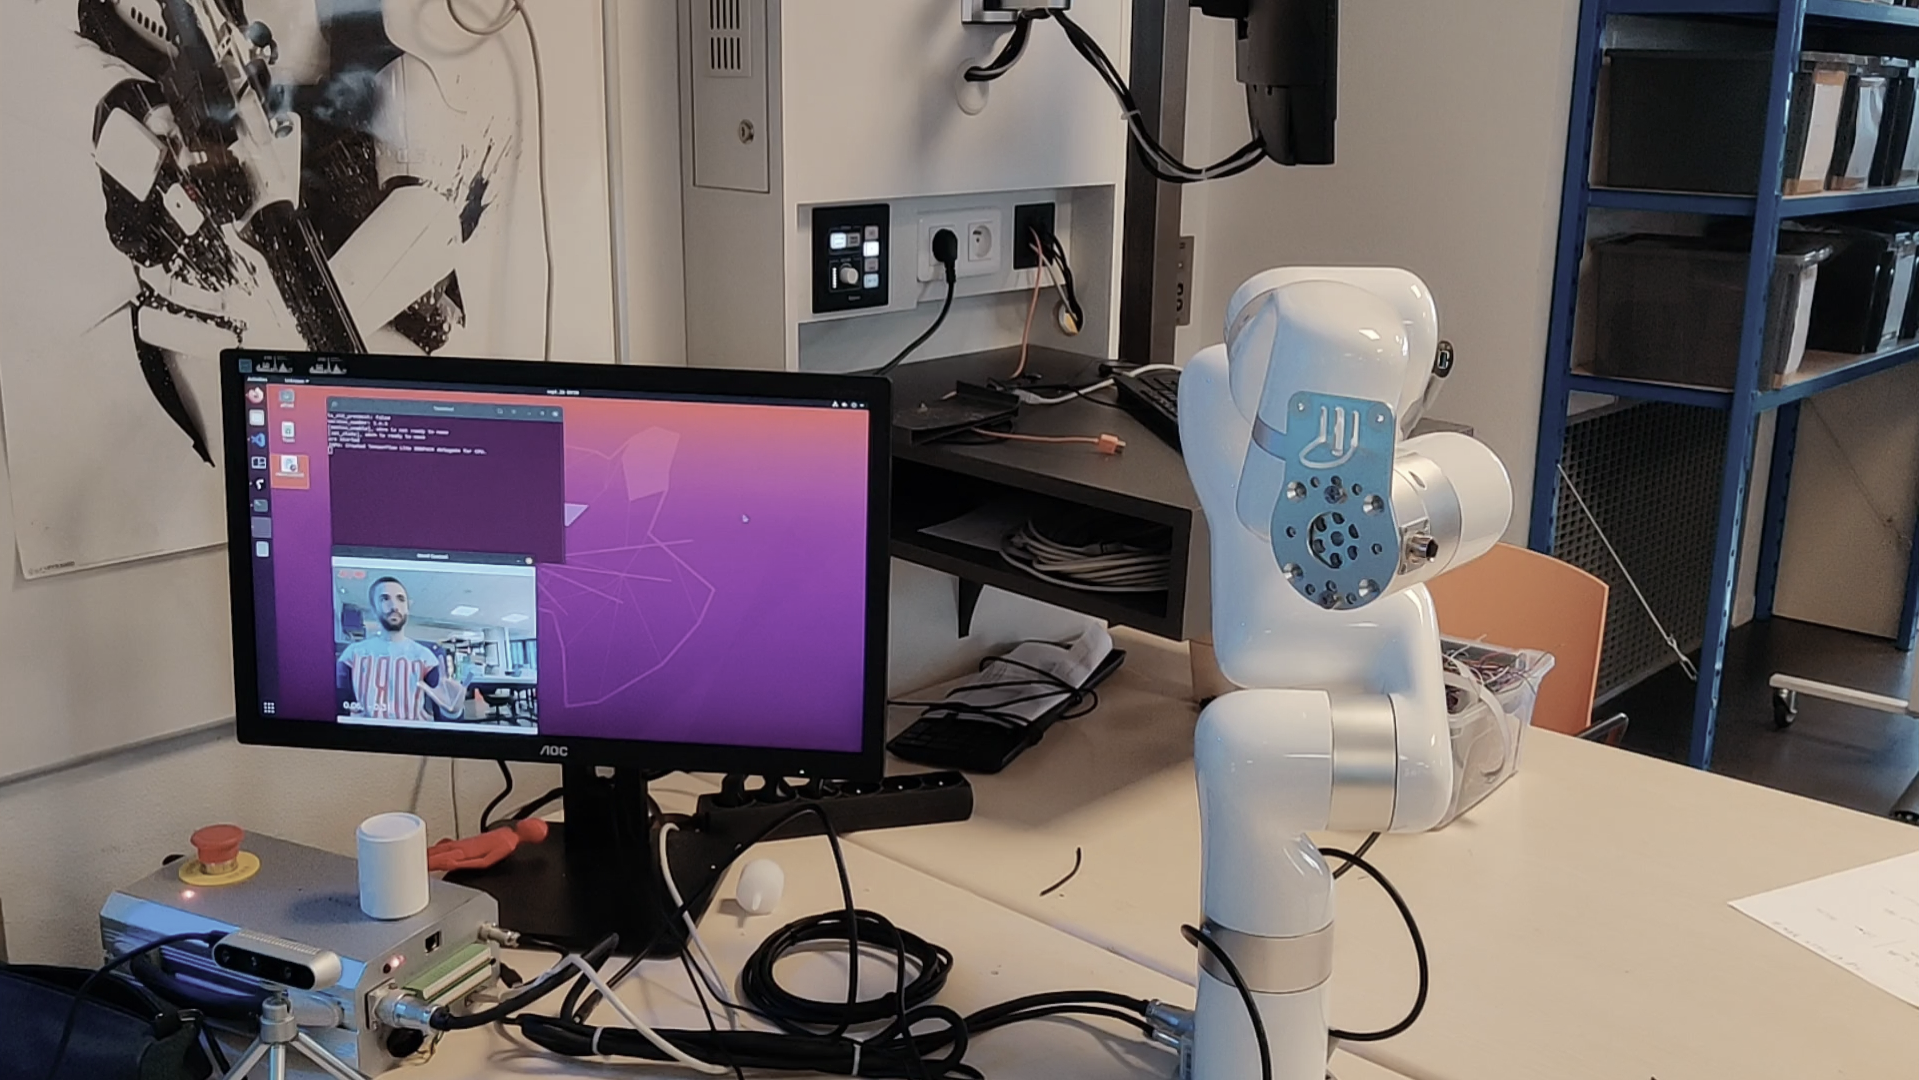
\includegraphics{images/hand_control_overview.png}
    \caption{Operating the arm with hand control. On the left, the computer running ALFRED with a camera pointed at the operator, showing the annotated camera feed. On the left, the robotic arm being controlled.}
    \label{fig:hand_control_overview}
\end{figure}

Hand control allows an operator to control the robotic arm with their hands \ref{fig:hand_control_overview}. It uses a camera pointed towards the operator and a hand recognition algorithm to detect the position of the hand. It then interprets the data to control the robotic arm. The hand control interface moves the robotic arm by comparing the position of the center of the hand\sidenote{Taken as the middle of the segment between the wrist and the index finger metacarpal} to the center of the video frame. If the hand is on the left of the center of the frame, the robot will move left (as seen from the front). The further away from the center the hand is, the faster the robot moves.

We trained machine and deep learning models to detect gestures which allow for further interaction, such as opening and closing a gripper, or starting and stopping other applications.

\subsubsection{Implementation}

Hand control has been implemented following the principle of dependency injection. The software contains only video processing, while video acquisition and moving the robotic arm itself are left to system developers. This allows modularity and adaptability for many, if not all, systems. In ALFRED, video acquisition is done through the drivers with a stream from the Pub/Sub abstracted by a class. Moving the robotic arm is done through a function injected into the Hand control software. The function takes in landmarks and gesture data from the model and translated them to robot commands specific to the robotic arm.

For the processing part itself, Hand control uses video frame data, hand detection, and post-processing to transform hand position into robotic arm commands. From frame data, hand detection is run using Mediapipe Hands\cite{mediapipe_hands}.

We extract 3D landmarks which represent the various points of interest on the hand. These landmarks represent the wrist and each finger joint, as well as each finger tip, for a total of 21 landmarks.

Two models were built to detect gestures from the landmarks. We built a dataset of hand gestures and their corresponding landmarks. The data was collected by taking a video of a subject doing the same hand gesture for a couple of seconds, moving and rotating their hand constantly and randomly. We only recorded the landmarks instead of the whole frames, so we only had 42 (21 landmarks, and x and y values for each landmark) values to record instead of the 640x480x3 values of the RGB frame. The data was augmented with small random rotations, as well as mirroring to enable generalization for both hands. We then trained a Random Forest using scikit-learn\cite{scikit-learn}, and a Multilayer Perceptron (MLP) implemented in PyTorch, with a few layers activated by the ReLU function.

From the hand landmarks, we create robot commands. Our initial command method was to create a linear mapping between the position of the hand and that of the robot's end effector. User feedback allowed us to finetune the method to be more intuitive and capable. This second method mimics the working of game controller joysticks. We transform the camera fram into the joystick: when the user moves their hand to the left of the frame, the robot moves continuously to the left. The speed of the movement is dependent on the distance between the center of the hand and the center of the frame.

The center of the frame contains a dead zone a couple of pixels in radius. When the user places their hand in this zone, no movement command will be issued. Gesture commands can still be recognized and issued. This was found to be necessary because the arm would make small movements when the user didn't want it to move. It would also add latency to the next movements: robot commands would be queued continuously and clog up the command queue.

To implement this control method, we compare the center of the hand to the center of the frame, and multiply the difference by an offset, found empirically (in our case, it is \lstinline{0.022}). The commands are then sent to move the robotic arm. The two methods are illustrated here \ref{fig:hand_control_methods}.

\begin{figure}
    \centering
    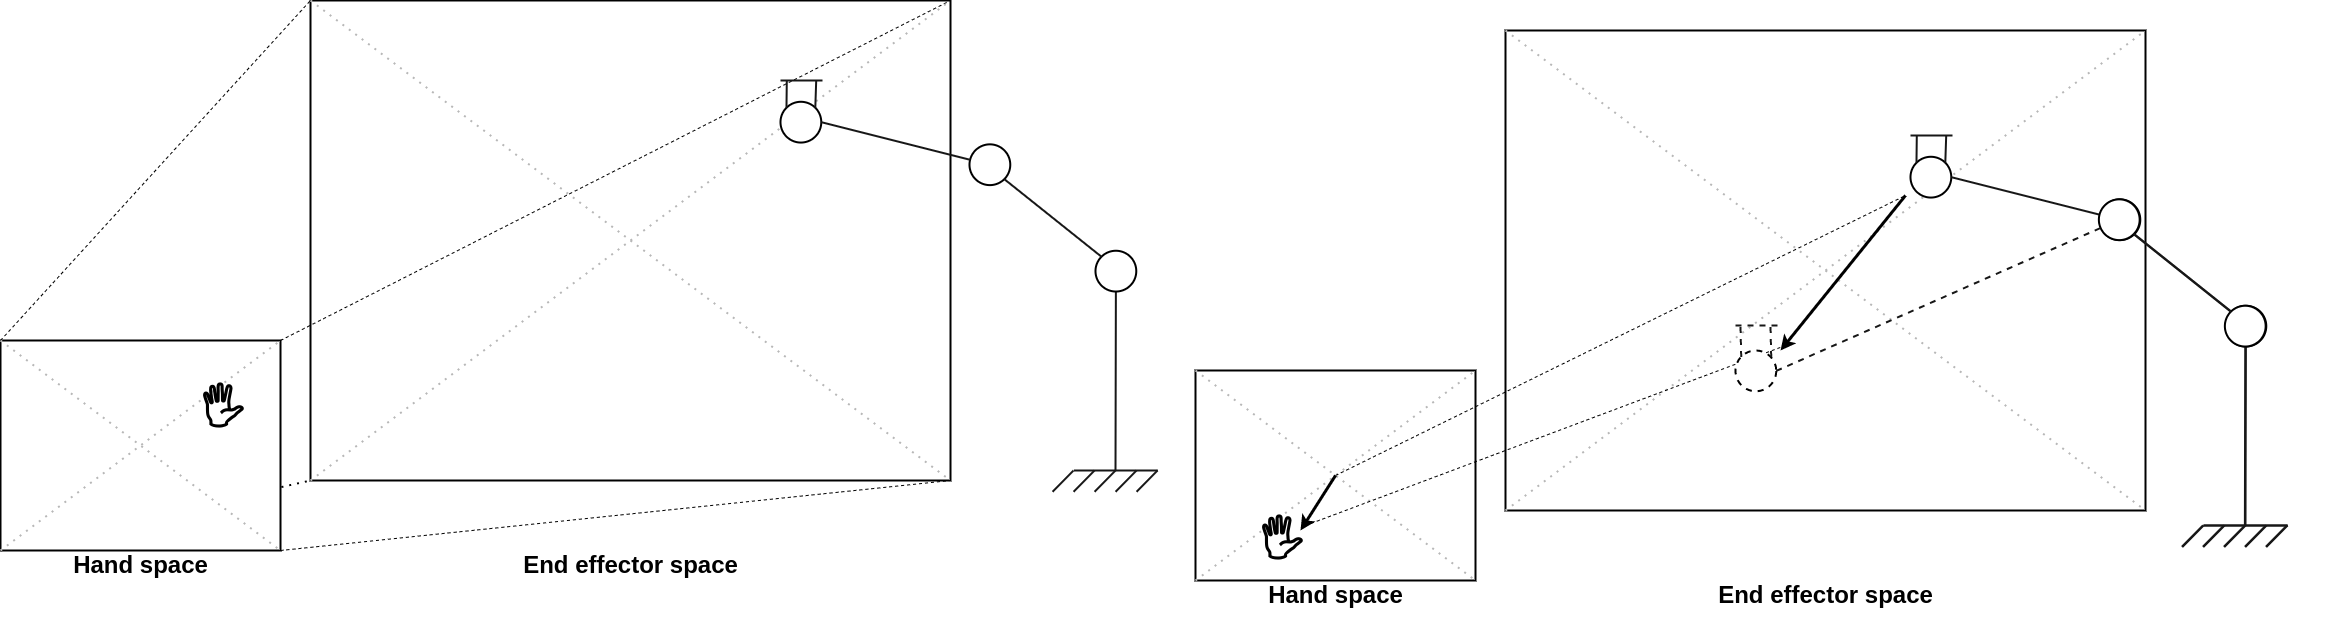
\includegraphics{images/hand_control_methods.png}
    \caption{First (left) and second (right) methods for translating hand position to robot command.}
    \label{fig:hand_control_methods}
\end{figure}


\subsubsection{Evaluation}

The goal of this interaction was to create a way to control a robotic arm that would be more intuitive than using gauges and dials on a computer screen. We selected four criteria to measure its effectiveness:

\begin{itemize}
    \item Intuitiveness: how natural it feels
    \item Usability: how good it feels to use
    \item Mobility: how it can move in its environment
    \item Precision: how difficult small movements are to achieve
\end{itemize}

We asked 8 participants to test the interaction. Of the 8, 5 had prior knowledge of the system and had at least a basic understanding of robotics, while the rest had no prior knowledge and no knowledge of robotics.

We used two tasks to evaluate our interaction:

\begin{itemize}
    \item Free exploration (intuitiveness, usability, mobility)
    \item Moving a plastic can balanced on top of a piece of wood (precision) \ref{fig:hand_control_task}
\end{itemize}

\begin{figure}[h]
    \centering
    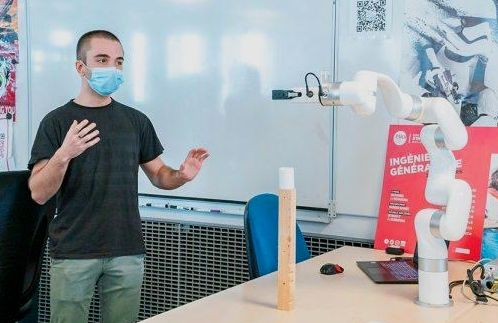
\includegraphics{images/hand_control_grasping.jpg}
    \caption{Preparing to grab the piece of wood to move the plastic can}
    \label{fig:hand_control_task}
\end{figure}

Free exploration was overall appreciated by the participants. It took them about five minutes to understand how the system works, which we found to be acceptable. Six out of the eight found the chosen method to be intuitive, and all the participants found it to be an effective method. There was one problem when starting the control session, specifically with the initial hand pose: the hand had to be perfectly centered or else the software would send the robot commands when it was still setting up, resulting in erratic movements that would sometimes break the system. Once aware of this problem, participants were able to avoid it reliably. The most limiting factor was range of motion, where the arm would make very big and fast movements when approaching the end of its operating zone. This would oftentimes break the software which would require a reboot. We can therefore validate intuitiveness and usability, but there needs to be further work on mobility by making further regions safer to operate in.

Our precision task used gestures, namely closing and opening the hand, to grab and release with the gripper robotic arm's gripper. The objective was to pick up and move a piece of wood with a 3D-printed soda can balanced on it in a circle, then put it back down. Four participants, all with prior knowledge, managed to complete the task, while the other four failed. Of the four that failed, two did because the gripper released the piece of wood too early, causing it to drop to the table. From this experiment, we can conclude that precision tasks required more trained operators, and that we had to improve the reliability of the system, specifically with hand gestures.


\subsection{Conclusion}

\subsubsection{Applications and use cases}

Hand movement and gesture control can be applied to any robotic arm to allow a minimally-trained operator to control the arm.

With this more natural method of control, as opposed to moving a slider or clicking on arrows, operators are able to achieve higher precision and a stronger connection between them and the robot.

More precise control for minimally trained operators means Hand movement and gesture control can be used by factory workers to move heavy weights, for example in a construction of metal factory, with a bigger industrial arm. It can also be used by researchers in laboratories, for moving dangerous pieces of equipment or chemicals during an experiment where hand manipulation, even through a glove box, would be risky. Finally, given the appropriate equipment, we could imagine a robotic arm moving through rough and dangerous terrain in rescue or cleanup operations.

\subsubsection{Limitations}

The main limitation for Hand movement and gesture control currently is the dimensionality: the arm can only be made to move in a plane. It cannot move in three dimensions which severely reduces its capabilities. Even more importantly, there is no way to rotate the arm. It will always be facing in the same orientation.

Secondly, using such a simple interface as the hand means that more advanced controls need to be hidden behind certain commands, or in our case gestures. This increases the complexity for understanding the system.

\subsubsection{Future works}

In the future, we would like to improve the system on the problems found in the user study and alleviate one of the limitations.

Mobility would be improved by creating safeguards around the edged of the range of motion to create smoother movements around these edges. Range of motion would be reduced a bit but to the benefit of more system reliability and easier handling because the system would not break or create sudden unplanned movements.

Grabbing reliability, or more generally gesture handling reliability, also needs improvement. Systems can be put in place to avoid suddenly releasing a grabbed object because of an error in gesture detection. For example, with buffering and outlier removal.

Another main aspect that would be improved is the dimensionality. While the arm can currently only be made to move in two dimensions (in a plane) with Hand movement control, we would like to make it move in three dimensions. This could be done by using depth frame data to measure the proximity of the hand to the camera. With some calibration at the beginning of handling, we could detect wether the operator moves their hand backwards or forwards, creating the possibility for the arm to move in the three dimensions.



\section{Vocal command control}


\subsection{Introduction}

Recent years have seen the rise of home assistants such as Siri from Apple or Alexa from Amazon. These assistants use complex deep learning algorithms to interpret the sound of your voice into commands to execute. These devices allow their users to control their home and automate tasks without having to touch anything. They act like a butler, constantly listening for requests and executing them when received.

We wanted to reproduce the same functionality for ALFRED: to allow users to talk to the platform as a means of interaction. Like home assistants, the objective was to create a "butler" that listens, like a human, to commands expressed in natural language, instead of pre-defined sentences. It would thus be more integrated into its environment as something almost living and intelligent.


% \subsection{Related work}

% % XXX: related_work


\subsection{Contribution}

\subsubsection{Concept}

Voice control allows an operator to control the robotic arm vocally. With data from the microphone driver, a Speech Recognition algorithm interprets the voice into text (Speech-To-Text, or STT). Text data is then interpreted by a Natural Language Processing (NLP) algorithm to extract intent and data from the command. From the intent, the system determines which API function to call, also sending the extracted data when necessary.

\subsubsection{Implementation}

We built a driver for microphones which provides raw audio data but is also capable of doing Speech-To-Text (STT). Using Azure Speech \cite{azure_speech}, we convert raw sound data (also from the driver) into text. We do continuous speech recognition: the STT model recognizes each word as it is spoken, and combines words together when a pause indicating the end of the sentence is detected. At the moment, only complete phrases are sent by the driver.

With the sentences detected by the STT part of the microphone driver, we run an NLP algorithm. Voice control uses RASA\cite{rasa}, a machine learning framework for building automation around text conversations. It uses Natural Language Understanding (NLU) to process text into intents and variables, which we call command data.

Intents are the purpose behind the sentence that was treated. Currently implemented intents include:

\begin{itemize}
    \item \lstinline{call}: Activate listening. Unless the system is called, it will not respond to commands, to avoid doing everything it hears against the operator's consent. Listening stays activated for a short period of time or until it is manually deactivated. An example of a sentence for this intent is: "Hey Alfred".
    \item \lstinline{uncall}: Deactivate listening. An example is: "Thank you Alfred".
    \item \lstinline{grab_object}: Grab the specified object. An example is: "Can you grab the cup ?"
    \item \lstinline{call+grab_object}: Associates the \lstinline{call} and \lstinline{grab_object} intents. An example is: "Hey Alfred, grab the bottle please".
\end{itemize}

Command data is a word or a set of words extracted from the command, that can change for the same intent. In the case of grabbing objects, data would be the object to grab. For example, in "Grab the pen please", RASA would extract the intent as "grab" and the data as "pen".

From the intent, the system determines which API function to call, also sending the extracted data when necessary.

% \subsubsection{Evaluation}


\subsection{Conclusion}

\subsubsection{Applications and use cases}

Voice control is used within ALFRED to interact with the system vocally. It allows users to manipulate the system in a natural manner, like talking to a human assistant. Voice control can also be integrated in other systems to make them controllable by voice. API routes can be mapped to voice control intents to make the system more accessible to users, in line with the objective of seamless integration.

Its applications can be imagined in makerspaces, as an interface for an automated personal assistant. The user could be doing a manual task and direct the assistant with their voice, in a natural manner. The user wouldn't need to put down their equipment to manipulate the assistant, and instead could continue doing their task in a seamless manner.

It could assist people who can't move their arms because of a disability who would have trouble controlling the robotic arm with a mouse and keyboard, or a controller, or even Hand and gesture control.

\subsubsection{Limitations}

Voice control is held back by its training complexity. Due to the nature of the software used, voice control cannot generalize easily for new commands or conversation paths. Each new intent needs dozens of training samples which need to be carefully selected, and each time the model must be re-trained and re-deployed. This makes it difficult for developers to extend Voice control with their specific use cases.

\subsubsection{Future works}

More intents and stories need to be developed to enable the Voice control software to be an autonomous assistant. Currently, it can only call functions from the robotics platform, but the goal is to make it more of an interface that can show the full capabilities of the platform, from listing all available features to describing the current state of the platform, or even to make tutorials and demonstrate how to do certain tasks with or without the robotic arm.



\section{Conclusion}

One of our objectives with ALFRED is to allow people to design interactions with a robotic arm and to provide the tools to facilitate doing so.

We explored the possibilities of ALFRED by creating two interactions of our own: hand movement and gesture control, and voice control. These interactions allowed us to finetune our system to make it more usable by future developers. When designing the interactions, we created services to enable the creation of the RASA server, a software unit that was not a driver, but also not a robotic application.

We discovered the idea of creating a connection between man and robot by mapping body parts to the robotic arm, and we searched for ways of translating body movements into robot commands that would feel natural to us humans.

Finally, deep learning was used to transform a simple robotic arm into a smart assistant and an integral part of the space it is located in.
